\section{Key-value server}
During the first four milestones, we were tasked with developing a distributed key-value storage system, which includes many features such as replication and caching. In this section, we focus on the implementation behind some of those properties.

\begin{figure}[h]
	\centering
	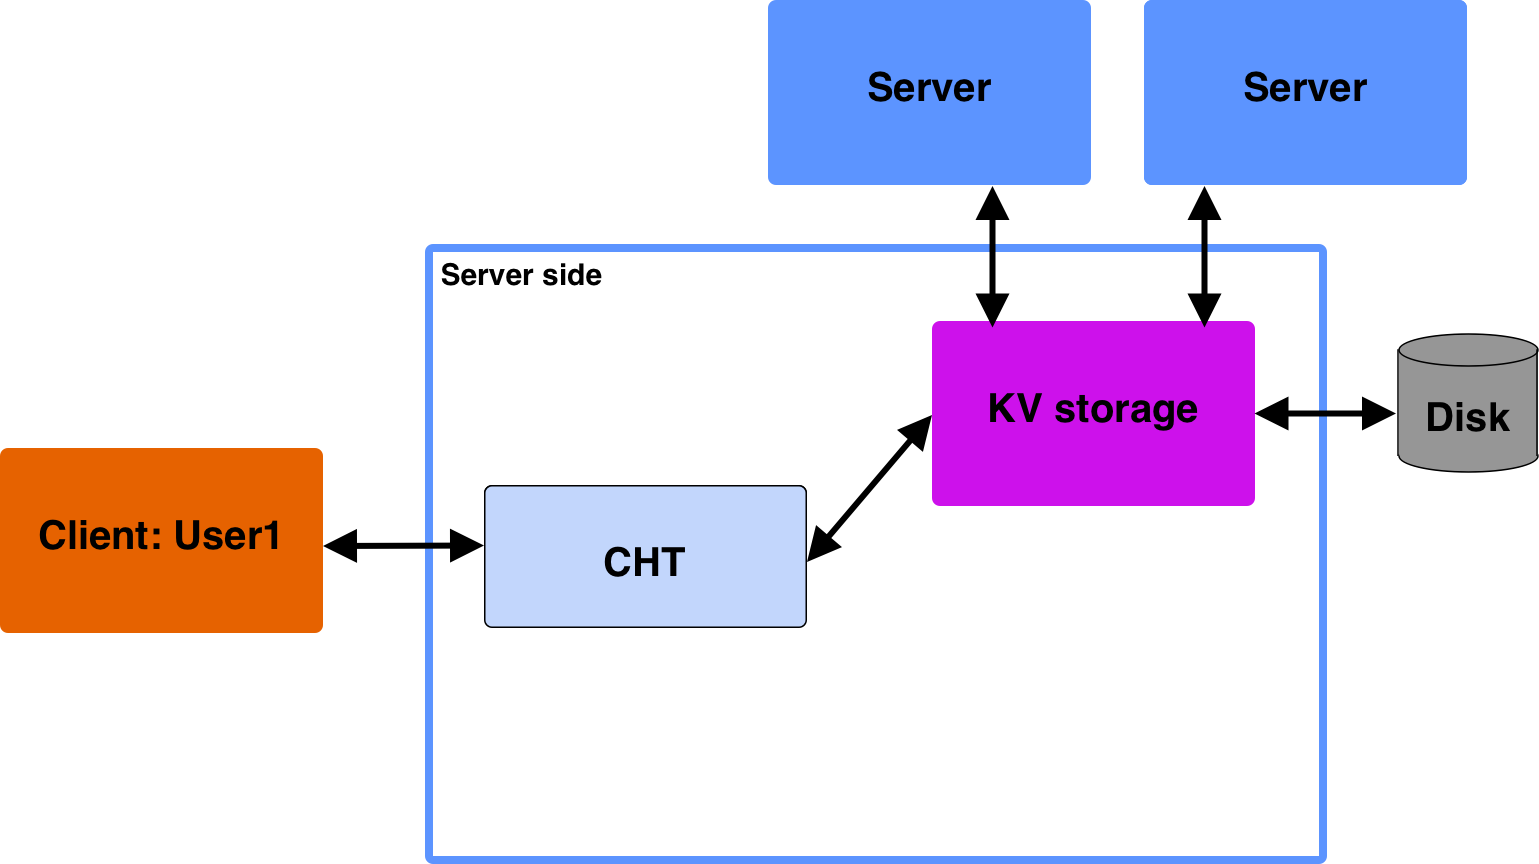
\includegraphics[width=\linewidth]{figures/kvserver/ms4_structure.png}
	\caption{KV server architecture}
\end{figure}




\begin{figure}[h]
	\centering
	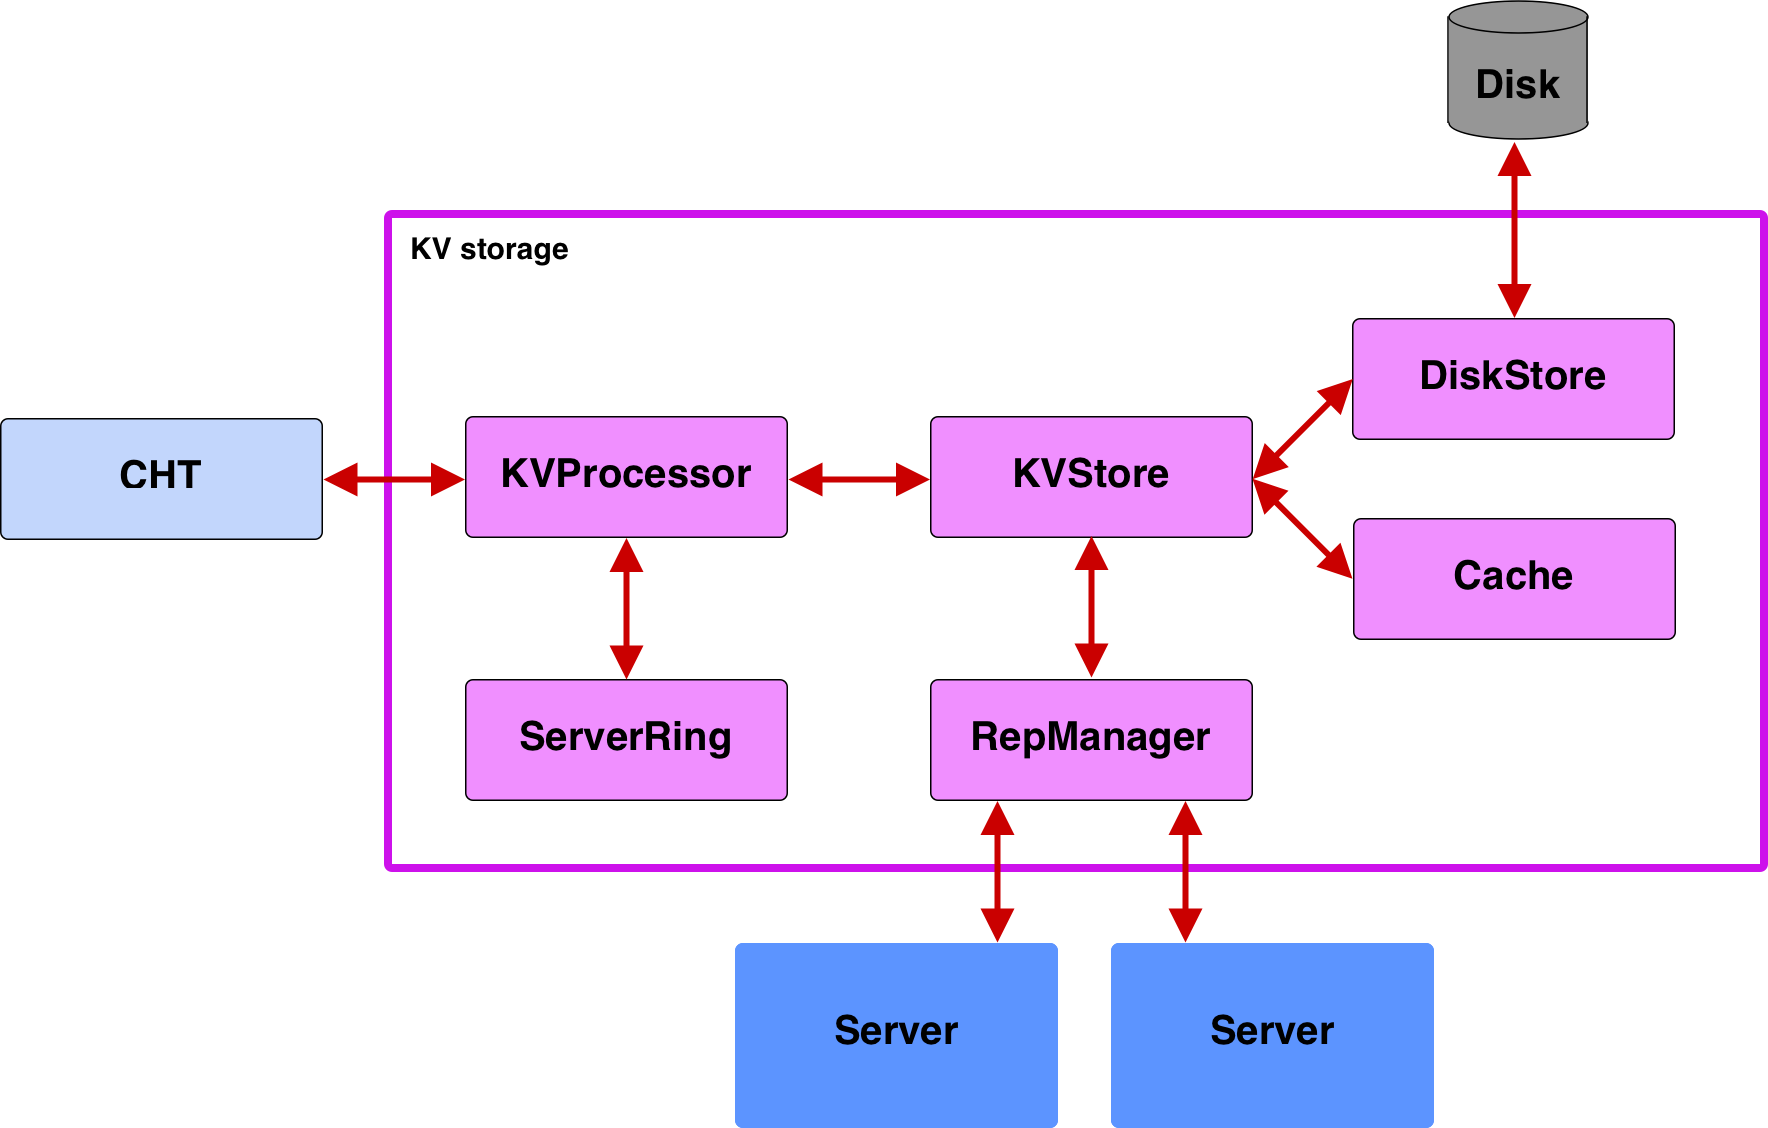
\includegraphics[width=\linewidth]{figures/kvserver/kvs_arch.png}
	\caption{Client side architecture}
\end{figure}


\subsection{Client Side Implementation}
\label{sec:Implementation_clintside}

\begin{figure}[h]
	\centering
	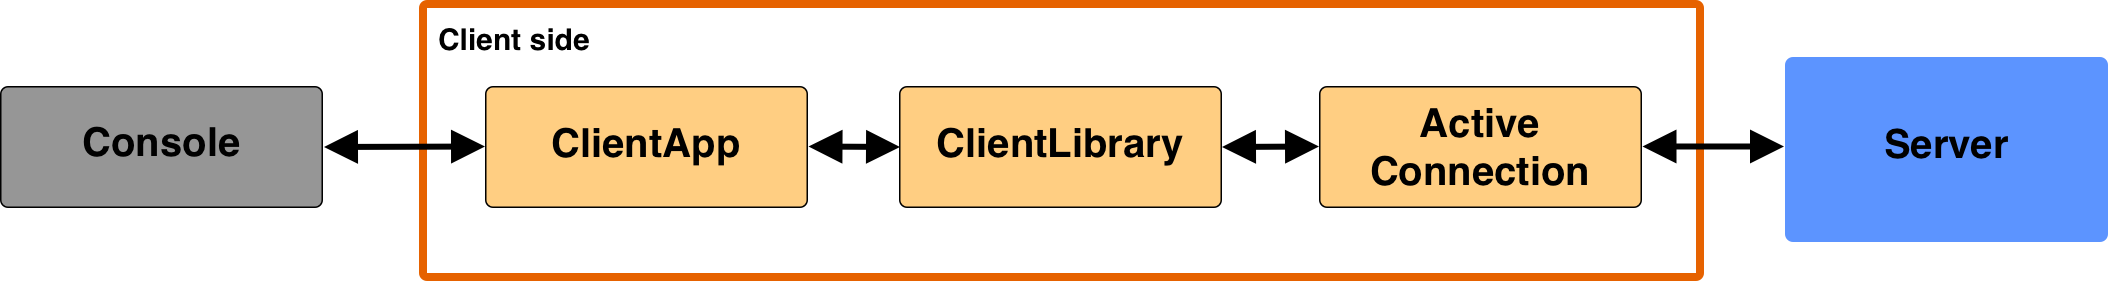
\includegraphics[width=\linewidth]{figures/kvserver/client_arch.png}
	\caption{Client side architecture}
	\label{fig:client_arch}
\end{figure}
The client side consists of the three following main components as seen in figure \ref{fig:client_arch}:
\begin{enumerate} 
  \item \textit{ClientApp} represents the client interface which allows input through the console. From there the client is able to issue commands to: connect to and disconnect from the system, interact with the key-value store and chat. The input is then checked and parsed before getting sent to the ClientLibrary. The result of the user command is displayed on the console through the ClientApp.
  \item \textit{ClientLibrary} serves as a bridge between the client and the server.
  \item \textit{ActiveConnection} abstracts the TCP socket connection to the server which allows the client to connect to the server socket and exchange data without worrying about the underlying structure.
\end{enumerate}
 
\subsection{Server Side Implementation}
\label{sec:implementation_serverside}

server side:
The client interacts directly only with the ConnectionHandleThread (CHT) created by the server to assist that specific client. The KV storage system provides the basic capabilities of a key-value store and persists data on disk. When more than two servers are online and replication is active, each server contains a replica of two other servers. Whenever a put operation is executed, it has to get forwarded to the server.

kv storage:
The KVCommandProcessor (KVCP) is responsible to receive commands from the CHT and return the result. Before a value is stored or retrieved, the KVCP utilizes the ServerRing to check whether the server is responsible for the provided key or not. In the latter case, a simple error message is returned back to the client, which would then connect to the responsible server. In the former case, the request is sent over to the KVStore. If it was a GET command issued, the KVStore first tries to retrieve the value from the cache. In case the value has not been found, the DiskStore checks if it is stored on disk.
With a PUT request, the KVStore sends the key-value pair to both the cache and DiskStore and also to the RepManager. This allows it to get sent over to the two replica servers. The RepManager is also charged with updating the replica on the server whenever one of the coordinators processes a PUT command.

